
\subsection{Draw}
$draw(f,x)$ draws a graph of the function $f$ of $x$.
The second argument can be omitted when the dependent variable
is literally $x$ or $t$.
The vectors $xrange$ and $yrange$ control the scale of the graph.

\begin{Verbatim}[formatcom=\color{blue}]
draw(x^2)
\end{Verbatim}

\begin{center}
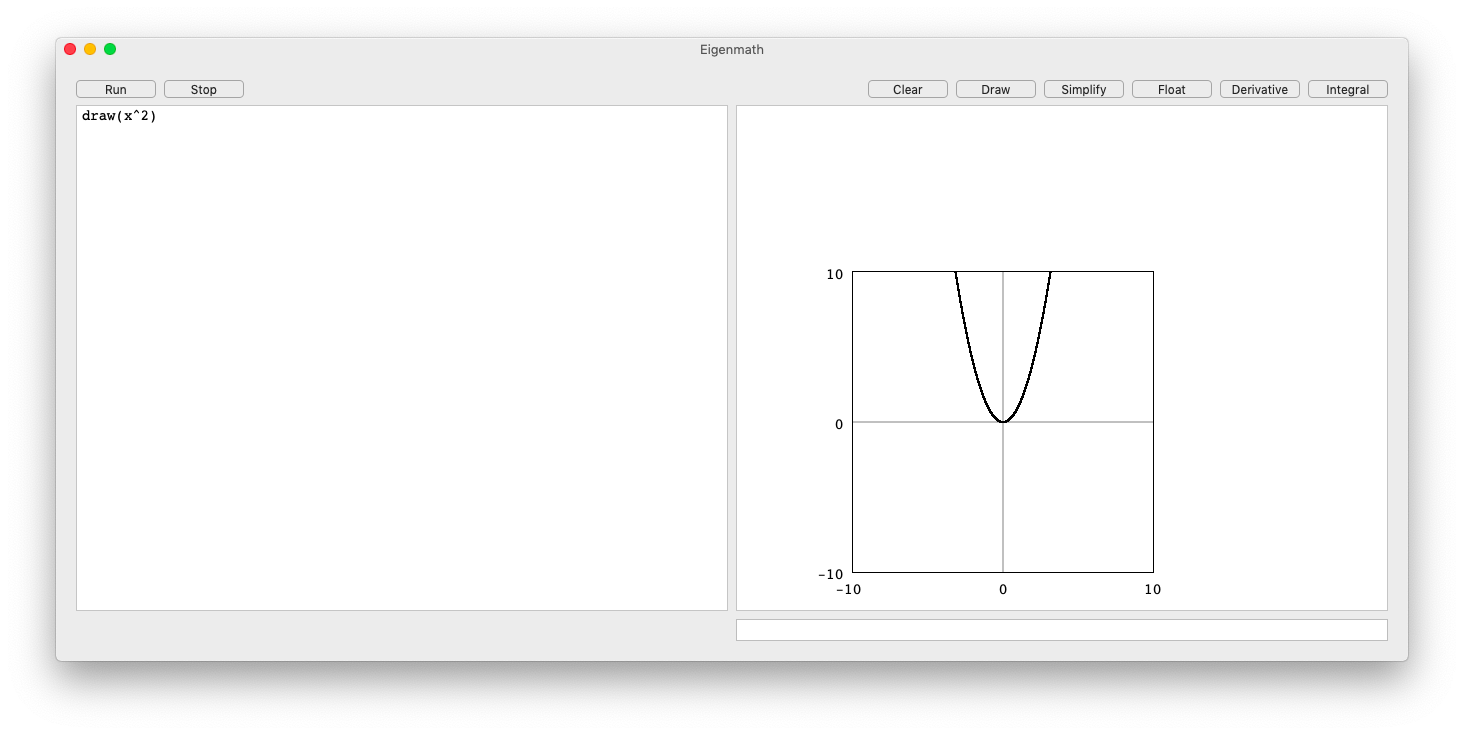
\includegraphics[scale=0.2]{parabola.png}
\end{center}

\begin{Verbatim}[formatcom=\color{blue},samepage=true]
xrange = (-1,1)
yrange = (0,2)
draw(x^2)
\end{Verbatim}

\begin{center}
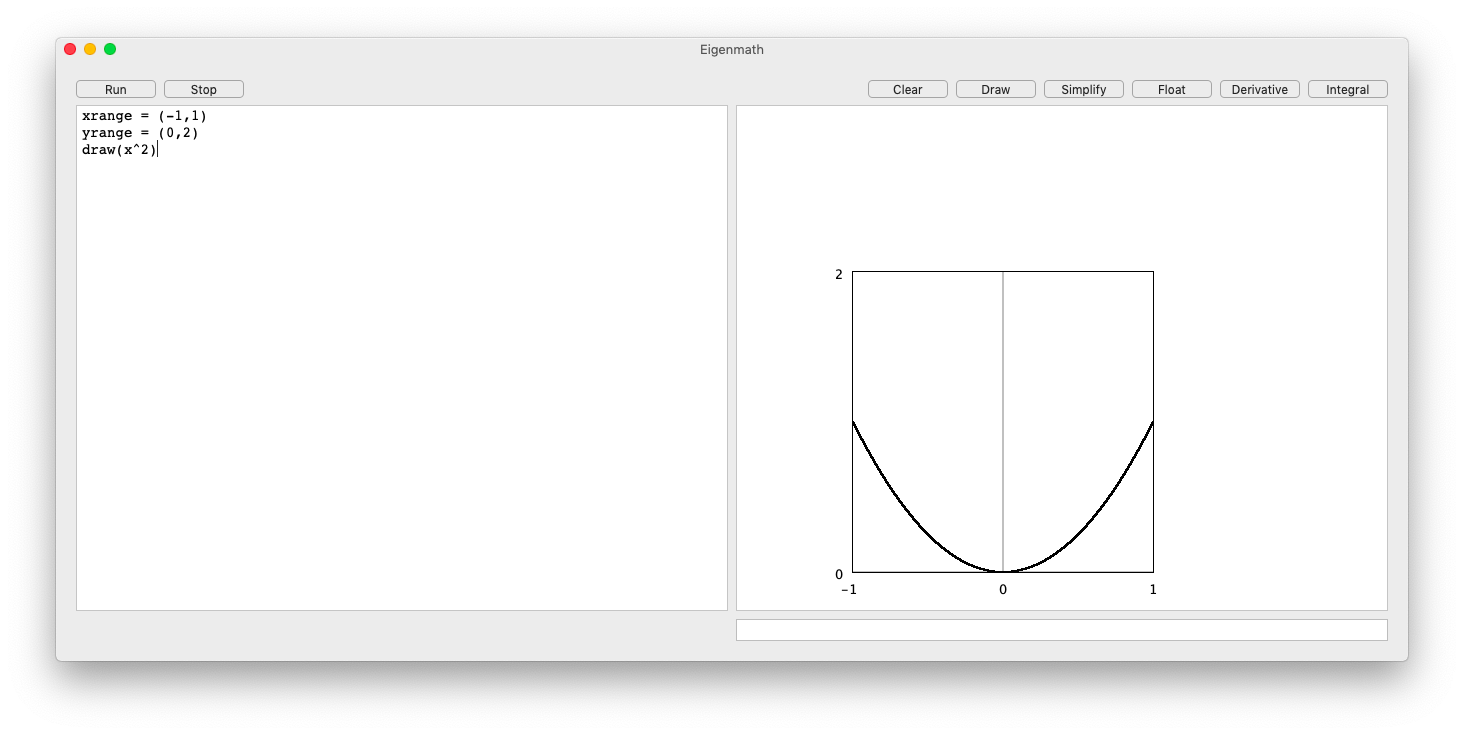
\includegraphics[scale=0.2]{parabola2.png}
\end{center}

Parametric drawing occurs when a function returns a vector.
The vector $trange$ controls the parametric range.
The default is $trange=(-\pi,\pi)$.
In the following example, $draw$ varies $theta$
over the default range $-\pi$ to $+\pi$.

\begin{Verbatim}[formatcom=\color{blue},samepage=true]
xrange = (-10,10)
yrange = (-10,10)
f = (cos(theta),sin(theta))
draw(5*f,theta)
\end{Verbatim}

\begin{center}
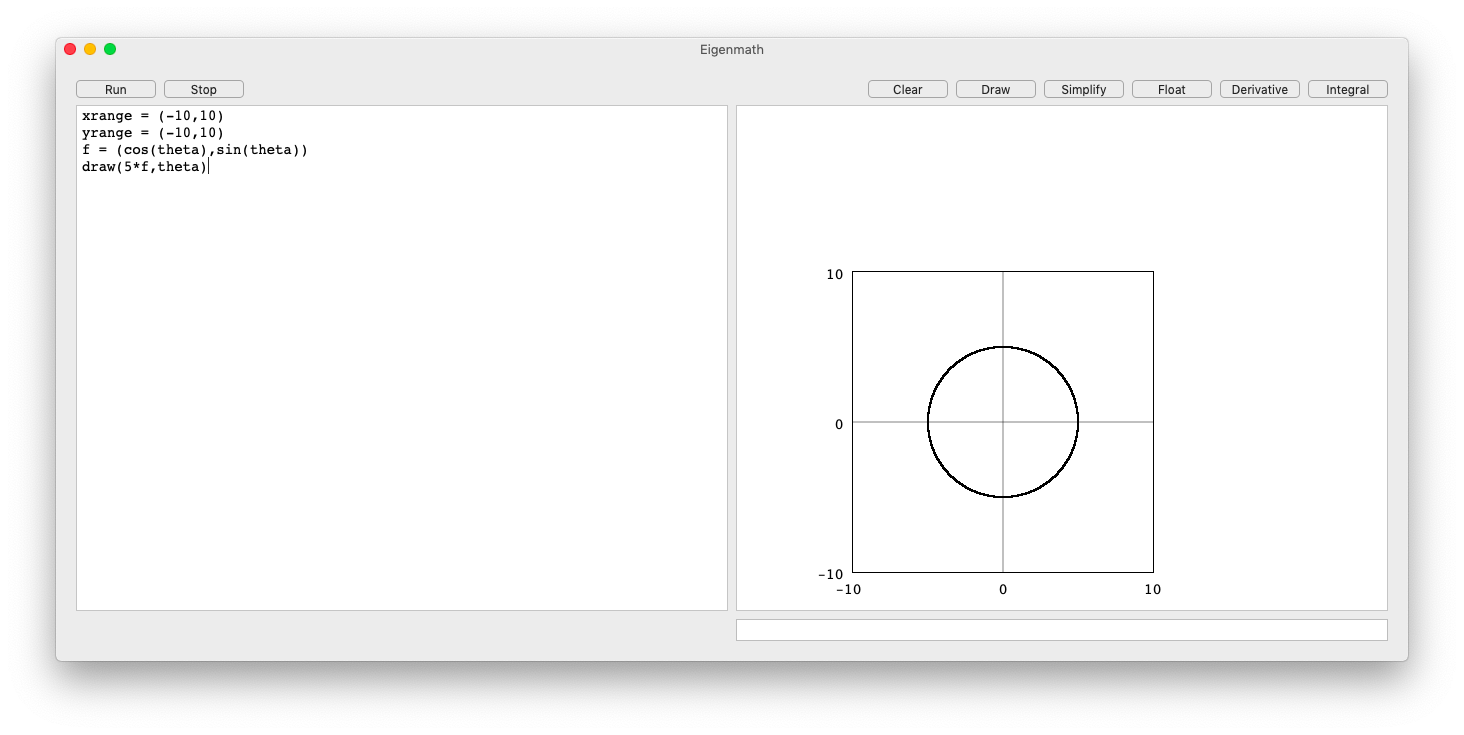
\includegraphics[scale=0.2]{circle.png}
\end{center}

In the following example, $trange$ is reduced
to draw a quarter circle instead of a full circle.

\begin{Verbatim}[formatcom=\color{blue},samepage=true]
trange = (0,pi/2)
f = (cos(theta),sin(theta))
draw(5*f,theta)
\end{Verbatim}

\begin{center}
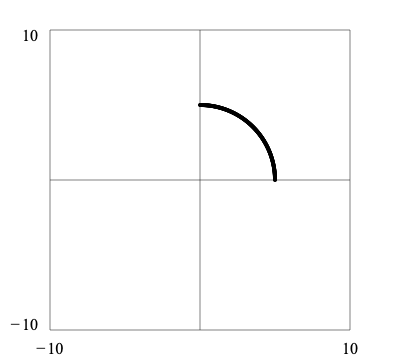
\includegraphics[scale=0.2]{circle2.png}
\end{center}

Here are a couple of interesting curves and the code for drawing them.
First is a lemniscate.

\begin{Verbatim}[formatcom=\color{blue},samepage=true]
trange = (-pi,pi)
X = cos(t)/(1+sin(t)^2)
Y = sin(t)*cos(t)/(1+sin(t)^2)
f = (X,Y)
draw(5*f,t)
\end{Verbatim}

\begin{center}
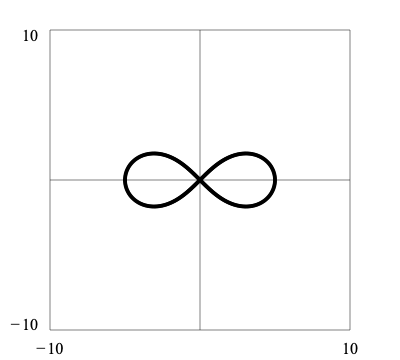
\includegraphics[scale=0.2]{lemniscate.png}
\end{center}

Next is a cardioid.

\begin{Verbatim}[formatcom=\color{blue},samepage=true]
r = (1+cos(t))/2
u = (cos(t),sin(t))
xrange = (-1,1)
yrange = (-1,1)
trange = (0,2*pi)
draw(r*u,t)
\end{Verbatim}

\begin{center}
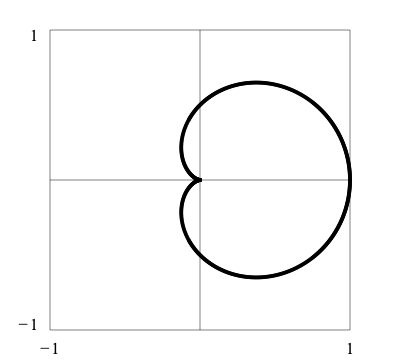
\includegraphics[scale=0.2]{cardioid.png}
\end{center}
